%------------------------------------------------------------------------------
\chapter{Ergebnisse der Störkörpermessungen}
\label{sec:appendix_felder}
%------------------------------------------------------------------------------

%------------------------------------------------------------------------------
\section{Elektrische Feldverteilung der $\mathrm{TM}_{010}$-Resonatormoden}
\label{app:tm010_felder}
%------------------------------------------------------------------------------
Im Folgenden werden die Feldverteilungen der vermessenen $\mathrm{TM}_{010}$-Resonatormoden der beiden Resonatoren PETRA-III und PETRA-IV zusammengetragen.
In allen Fällen ist die Position~$z$ relativ zum Vakuumflansch des Resonators und die elektrischen Felder normiert auf die Wurzel der Verlustleistung~$P_\mathrm{V}$ angegeben.

\subsection{PETRA-III}
\FloatBarrier
\begin{figure}[h]
  \centering
  \input{./plots/PETRA-III/pi.tex}
  \caption[Feldverteilung der $\mathrm{TM}_{010}\text{-}\pi$-Mode von PETRA-III]{Feldverteilung der $\mathrm{TM}_{010}\text{-}\pi$-Mode von PETRA-III bei einer Resonanzfrequenz von \mbox{$\nu_0 = \SI{499.67}{MHz}$} im Vakuum.}
\end{figure}

\begin{figure}[p]
	\centering
	
	\input{./plots/PETRA-III/2_3_pi.tex}
	\caption[Feldverteilung der $\mathrm{TM}_{010}\text{-}\frac{2}{3}\pi$-Mode von PETRA-III]{Feldverteilung der $\mathrm{TM}_{010}\text{-}\frac{2}{3}\pi$-Mode von PETRA-III bei einer Resonanzfrequenz von \mbox{$\nu_0 = \SI{501.14}{MHz}$} im Vakuum.}
	
	\input{./plots/PETRA-III/1_3_pi.tex}
	\caption[Feldverteilung der $\mathrm{TM}_{010}\text{-}\frac{1}{3}\pi$-Mode von PETRA-III]{Feldverteilung der $\mathrm{TM}_{010}\text{-}\frac{1}{3}\pi$-Mode von PETRA-III bei einer Resonanzfrequenz von \mbox{$\nu_0 = \SI{505.37}{MHz}$} im Vakuum.}
\end{figure}

\begin{figure}[p]
  \centering
  \input{./plots/PETRA-III/0_pi.tex}
  \caption[Feldverteilung der $\mathrm{TM}_{010}\text{-}0$-Mode von PETRA-III]{Feldverteilung der $\mathrm{TM}_{010}\text{-}0$-Mode von PETRA-III bei einer Resonanzfrequenz von \mbox{$\nu_0 = \SI{508.61}{MHz}$} im Vakuum.}
\end{figure}
\FloatBarrier

\clearpage
\subsection{PETRA-IV}
\FloatBarrier
\begin{figure}[h]
  \centering
  \input{./plots/PETRA-IV/pi.tex}
  \caption[Feldverteilung der $\mathrm{TM}_{010}\text{-}\pi$-Mode von PETRA-IV]{Feldverteilung der $\mathrm{TM}_{010}\text{-}\pi$-Mode von PETRA-IV bei einer Resonanzfrequenz von \mbox{$\nu_0 = \SI{499.67}{MHz}$} im Vakuum.}
\end{figure}

\begin{figure}[p]
	\centering
  
	\input{./plots/PETRA-IV/2_3_pi.tex}
	\caption[Feldverteilung der $\mathrm{TM}_{010}\text{-}\frac{2}{3}\pi$-Mode von PETRA-IV]{Feldverteilung der $\mathrm{TM}_{010}\text{-}\frac{2}{3}\pi$-Mode von PETRA-IV bei einer Resonanzfrequenz von \mbox{$\nu_0 = \SI{501.17}{MHz}$} im Vakuum.}
	
    \input{./plots/PETRA-IV/1_3_pi.tex}
    \caption[Feldverteilung der $\mathrm{TM}_{010}\text{-}\frac{1}{3}\pi$-Mode von PETRA-IV]{Feldverteilung der $\mathrm{TM}_{010}\text{-}\frac{1}{3}\pi$-Mode von PETRA-IV bei einer Resonanzfrequenz von \mbox{$\nu_0 = \SI{505.43}{MHz}$} im Vakuum.}
\end{figure}

\begin{figure}[h]
  \centering
  \input{./plots/PETRA-IV/0_pi.tex}
  \caption[Feldverteilung der $\mathrm{TM}_{010}\text{-}0$-Mode von PETRA-IV]{Feldverteilung der $\mathrm{TM}_{010}\text{-}0$-Mode von PETRA-IV bei einer Resonanzfrequenz von \mbox{$\nu_0 = \SI{508.61}{MHz}$} im Vakuum.}
\end{figure}
\FloatBarrier

\clearpage
%------------------------------------------------------------------------------
\section{Elektrische Feldverteilung von Resonatormoden höherer Ordnung}
\label{app:hom_felder}
%------------------------------------------------------------------------------
\FloatBarrier
Im Folgenden werden die Feldverteilungen der vermessenen Moden höherer Ordnung des Resonators PETRA-III zusammengetragen.
In allen Fällen ist die Position~$z$ relativ zum Vakuumflansch des Resonators und die elektrischen Felder normiert auf die Wurzel der Verlustleistung~$P_\mathrm{V}$ angegeben.
\begin{figure}[h]
  \centering
  \input{./plots/HOM/702MHz.tex}
  \caption[Transversale Feldverteilung der $\mathrm{TE}_{111}$-Mode \mbox{$\nu_0 = \SI{702.70}{MHz}$}]{Transversale Feldverteilung der $\mathrm{TE}_{111}$-Mode bei einer Resonanzfrequenz von \mbox{$\nu_0 = \SI{702.70}{MHz}$} im Vakuum.}
\end{figure}

\begin{figure}[p]
	\centering
	
	\input{./plots/HOM/730MHz.tex}
	\caption[Longitudinale Feldverteilung der $\mathrm{TM}_{011}$-Mode \mbox{$\nu_0 = \SI{730.45}{MHz}$}]{Longitudinale Feldverteilung der $\mathrm{TM}_{011}$-Mode bei einer Resonanzfrequenz von \mbox{$\nu_0 = \SI{730.45}{MHz}$} im Vakuum.}
	
	\input{./plots/HOM/1047MHz.tex}
	\caption[Transversale Feldverteilung der $\mathrm{TM}_{111}$-Mode \mbox{$\nu_0 = \SI{1047.23}{MHz}$}]{Transversale Feldverteilung der $\mathrm{TM}_{111}$-Mode bei einer Resonanzfrequenz von \mbox{$\nu_0 = \SI{1047.23}{MHz}$} im Vakuum.}
\end{figure}

\begin{figure}[p]
	\centering
	
	\input{./plots/HOM/1375MHz.tex}
	\caption[Longitudinale Feldverteilung der Mode \mbox{$\nu_0 = \SI{1375.79}{MHz}$}]{Longitudinale Feldverteilung der Mode bei einer Resonanzfrequenz von \mbox{$\nu_0 = \SI{1375.79}{MHz}$} im Vakuum.}
	
    \input{./plots/HOM/1458MHz.tex}
    \caption[Longitudinale Feldverteilung der $\mathrm{TM}_{021}$-Mode \mbox{$\nu_0 = \SI{1458.30}{MHz}$}]{Longitudinale Feldverteilung der $\mathrm{TM}_{021}$-Mode bei einer Resonanzfrequenz von \mbox{$\nu_0 = \SI{1458.30}{MHz}$} im Vakuum.}
\end{figure}

\begin{figure}[p]
	\centering
	\input{./plots/HOM/1460MHz.tex}
	\caption[Longitudinale Feldverteilung der $\mathrm{TM}_{021}$-Mode \mbox{$\nu_0 = \SI{1460.34}{MHz}$}]{Longitudinale Feldverteilung der $\mathrm{TM}_{021}$-Mode bei einer Resonanzfrequenz von \mbox{$\nu_0 = \SI{1460.34}{MHz}$} im Vakuum.}
	
    % GNUPLOT: LaTeX picture with Postscript
\begingroup
  \makeatletter
  \providecommand\color[2][]{%
    \GenericError{(gnuplot) \space\space\space\@spaces}{%
      Package color not loaded in conjunction with
      terminal option `colourtext'%
    }{See the gnuplot documentation for explanation.%
    }{Either use 'blacktext' in gnuplot or load the package
      color.sty in LaTeX.}%
    \renewcommand\color[2][]{}%
  }%
  \providecommand\includegraphics[2][]{%
    \GenericError{(gnuplot) \space\space\space\@spaces}{%
      Package graphicx or graphics not loaded%
    }{See the gnuplot documentation for explanation.%
    }{The gnuplot epslatex terminal needs graphicx.sty or graphics.sty.}%
    \renewcommand\includegraphics[2][]{}%
  }%
  \providecommand\rotatebox[2]{#2}%
  \@ifundefined{ifGPcolor}{%
    \newif\ifGPcolor
    \GPcolortrue
  }{}%
  \@ifundefined{ifGPblacktext}{%
    \newif\ifGPblacktext
    \GPblacktexttrue
  }{}%
  % define a \g@addto@macro without @ in the name:
  \let\gplgaddtomacro\g@addto@macro
  % define empty templates for all commands taking text:
  \gdef\gplbacktext{}%
  \gdef\gplfronttext{}%
  \makeatother
  \ifGPblacktext
    % no textcolor at all
    \def\colorrgb#1{}%
    \def\colorgray#1{}%
  \else
    % gray or color?
    \ifGPcolor
      \def\colorrgb#1{\color[rgb]{#1}}%
      \def\colorgray#1{\color[gray]{#1}}%
      \expandafter\def\csname LTw\endcsname{\color{white}}%
      \expandafter\def\csname LTb\endcsname{\color{black}}%
      \expandafter\def\csname LTa\endcsname{\color{black}}%
      \expandafter\def\csname LT0\endcsname{\color[rgb]{1,0,0}}%
      \expandafter\def\csname LT1\endcsname{\color[rgb]{0,1,0}}%
      \expandafter\def\csname LT2\endcsname{\color[rgb]{0,0,1}}%
      \expandafter\def\csname LT3\endcsname{\color[rgb]{1,0,1}}%
      \expandafter\def\csname LT4\endcsname{\color[rgb]{0,1,1}}%
      \expandafter\def\csname LT5\endcsname{\color[rgb]{1,1,0}}%
      \expandafter\def\csname LT6\endcsname{\color[rgb]{0,0,0}}%
      \expandafter\def\csname LT7\endcsname{\color[rgb]{1,0.3,0}}%
      \expandafter\def\csname LT8\endcsname{\color[rgb]{0.5,0.5,0.5}}%
    \else
      % gray
      \def\colorrgb#1{\color{black}}%
      \def\colorgray#1{\color[gray]{#1}}%
      \expandafter\def\csname LTw\endcsname{\color{white}}%
      \expandafter\def\csname LTb\endcsname{\color{black}}%
      \expandafter\def\csname LTa\endcsname{\color{black}}%
      \expandafter\def\csname LT0\endcsname{\color{black}}%
      \expandafter\def\csname LT1\endcsname{\color{black}}%
      \expandafter\def\csname LT2\endcsname{\color{black}}%
      \expandafter\def\csname LT3\endcsname{\color{black}}%
      \expandafter\def\csname LT4\endcsname{\color{black}}%
      \expandafter\def\csname LT5\endcsname{\color{black}}%
      \expandafter\def\csname LT6\endcsname{\color{black}}%
      \expandafter\def\csname LT7\endcsname{\color{black}}%
      \expandafter\def\csname LT8\endcsname{\color{black}}%
    \fi
  \fi
    \setlength{\unitlength}{0.0500bp}%
    \ifx\gptboxheight\undefined%
      \newlength{\gptboxheight}%
      \newlength{\gptboxwidth}%
      \newsavebox{\gptboxtext}%
    \fi%
    \setlength{\fboxrule}{0.5pt}%
    \setlength{\fboxsep}{1pt}%
\begin{picture}(8502.00,5668.00)%
    \gplgaddtomacro\gplbacktext{%
      \csname LTb\endcsname%
      \put(1078,704){\makebox(0,0)[r]{\strut{}-2500}}%
      \csname LTb\endcsname%
      \put(1078,1174){\makebox(0,0)[r]{\strut{}-2000}}%
      \csname LTb\endcsname%
      \put(1078,1644){\makebox(0,0)[r]{\strut{}-1500}}%
      \csname LTb\endcsname%
      \put(1078,2114){\makebox(0,0)[r]{\strut{}-1000}}%
      \csname LTb\endcsname%
      \put(1078,2584){\makebox(0,0)[r]{\strut{}-500}}%
      \csname LTb\endcsname%
      \put(1078,3054){\makebox(0,0)[r]{\strut{}0}}%
      \csname LTb\endcsname%
      \put(1078,3523){\makebox(0,0)[r]{\strut{}500}}%
      \csname LTb\endcsname%
      \put(1078,3993){\makebox(0,0)[r]{\strut{}1000}}%
      \csname LTb\endcsname%
      \put(1078,4463){\makebox(0,0)[r]{\strut{}1500}}%
      \csname LTb\endcsname%
      \put(1078,4933){\makebox(0,0)[r]{\strut{}2000}}%
      \csname LTb\endcsname%
      \put(1078,5403){\makebox(0,0)[r]{\strut{}2500}}%
      \csname LTb\endcsname%
      \put(1210,484){\makebox(0,0){\strut{}0}}%
      \csname LTb\endcsname%
      \put(2763,484){\makebox(0,0){\strut{}500}}%
      \csname LTb\endcsname%
      \put(4316,484){\makebox(0,0){\strut{}1000}}%
      \csname LTb\endcsname%
      \put(5869,484){\makebox(0,0){\strut{}1500}}%
      \csname LTb\endcsname%
      \put(7422,484){\makebox(0,0){\strut{}2000}}%
    }%
    \gplgaddtomacro\gplfronttext{%
      \csname LTb\endcsname%
      \put(176,3053){\rotatebox{-270}{\makebox(0,0){\strut{}$\frac{E_0(z)}{\sqrt{P_\mathrm{V}}}$ / \si{\volt\per\metre\per\watt\tothe{0.5}}}}}%
      \put(4657,154){\makebox(0,0){\strut{}$z$ / \si{mm}}}%
      \csname LTb\endcsname%
      \put(7382,5230){\makebox(0,0)[r]{\strut{}Amplitude}}%
      \csname LTb\endcsname%
      \put(7382,5010){\makebox(0,0)[r]{\strut{}effektives Feld}}%
    }%
    \gplbacktext
    \put(0,0){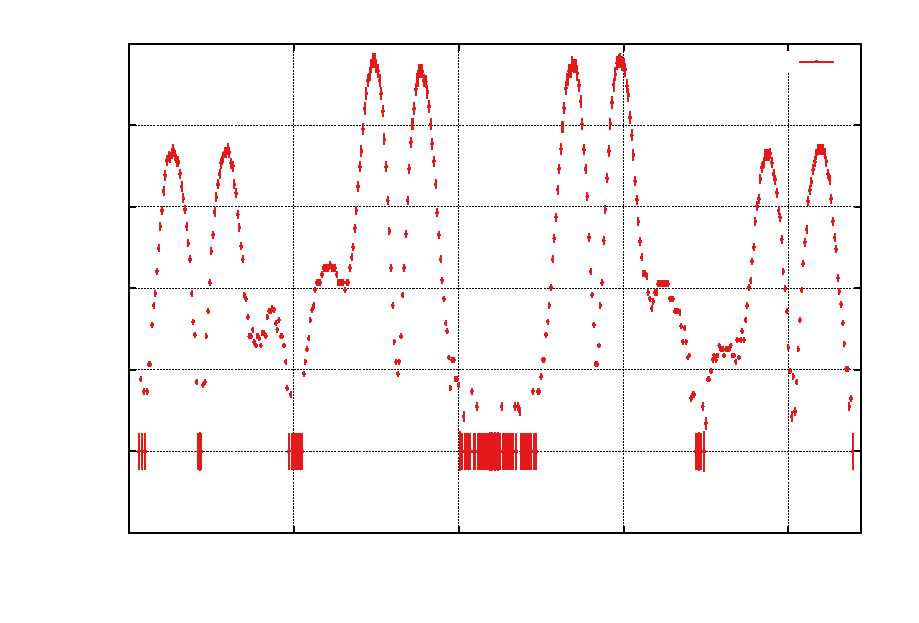
\includegraphics{./plots/HOM/1465_L_MHz}}%
    \gplfronttext
  \end{picture}%
\endgroup

    \caption[Longitudinale Feldverteilung der $\mathrm{TM}_{021}$-Mode \mbox{$\nu_0 = \SI{1464.96}{MHz}$}]{Longitudinale Feldverteilung der $\mathrm{TM}_{021}$-Mode bei einer Resonanzfrequenz von \mbox{$\nu_0 = \SI{1464.96}{MHz}$} im Vakuum.}
\end{figure}


\begin{figure}[p]
  \centering
  \input{./plots/HOM/1465_R_MHz.tex}
  \caption[Longitudinale Feldverteilung der $\mathrm{TM}_{021}$-Mode \mbox{$\nu_0 = \SI{1465.83}{MHz}$}]{Longitudinale Feldverteilung der $\mathrm{TM}_{021}$-Mode bei einer Resonanzfrequenz von \mbox{$\nu_0 = \SI{1465.83}{MHz}$} im Vakuum.}
\end{figure}


\FloatBarrier